%%%%%%%%%%%%%%%%%%%%%%%%%%%%%%%%%%%%%%%%%
% Lachaise Assignment
% LaTeX Template
% Version 1.0 (26/6/2018)
%
% This template originates from:
% http://www.LaTeXTemplates.com
%
% Authors:
% Marion Lachaise & François Févotte
% Vel (vel@LaTeXTemplates.com)
%
% License:
% CC BY-NC-SA 3.0 (http://creativecommons.org/licenses/by-nc-sa/3.0/)
%
%%%%%%%%%%%%%%%%%%%%%%%%%%%%%%%%%%%%%%%%%

%----------------------------------------------------------------------------------------
%	PACKAGES AND OTHER DOCUMENT CONFIGURATIONS
%----------------------------------------------------------------------------------------

\documentclass{article}

%%%%%%%%%%%%%%%%%%%%%%%%%%%%%%%%%%%%%%%%%
% Lachaise Assignment
% Structure Specification File
% Version 1.0 (26/6/2018)
%
% This template originates from:
% http://www.LaTeXTemplates.com
%
% Authors:
% Marion Lachaise & François Févotte
% Vel (vel@LaTeXTemplates.com)
%
% License:
% CC BY-NC-SA 3.0 (http://creativecommons.org/licenses/by-nc-sa/3.0/)
% 
%%%%%%%%%%%%%%%%%%%%%%%%%%%%%%%%%%%%%%%%%

%----------------------------------------------------------------------------------------
%	PACKAGES AND OTHER DOCUMENT CONFIGURATIONS
%----------------------------------------------------------------------------------------

\usepackage{amsmath,amsfonts,stmaryrd,amssymb} % Math packages

\usepackage{enumerate} % Custom item numbers for enumerations

\usepackage[ruled]{algorithm2e} % Algorithms

\usepackage[framemethod=tikz]{mdframed} % Allows defining custom boxed/framed environments

\usepackage{graphicx} % images

\usepackage{hyperref}
\graphicspath{ {../code/outputs/} }

\usepackage{listings} % File listings, with syntax highlighting
\lstset{
	basicstyle=\ttfamily, % Typeset listings in monospace font
}

%----------------------------------------------------------------------------------------
%	DOCUMENT MARGINS
%----------------------------------------------------------------------------------------

\usepackage{geometry} % Required for adjusting page dimensions and margins

\geometry{
	paper=a4paper, % Paper size, change to letterpaper for US letter size
	top=2.5cm, % Top margin
	bottom=3cm, % Bottom margin
	left=2.5cm, % Left margin
	right=2.5cm, % Right margin
	headheight=14pt, % Header height
	footskip=1.5cm, % Space from the bottom margin to the baseline of the footer
	headsep=1.2cm, % Space from the top margin to the baseline of the header
	%showframe, % Uncomment to show how the type block is set on the page
}

%----------------------------------------------------------------------------------------
%	FONTS
%----------------------------------------------------------------------------------------

\usepackage[utf8]{inputenc} % Required for inputting international characters
\usepackage[T1]{fontenc} % Output font encoding for international characters

\usepackage{XCharter} % Use the XCharter fonts

%----------------------------------------------------------------------------------------
%	COMMAND LINE ENVIRONMENT
%----------------------------------------------------------------------------------------

% Usage:
% \begin{commandline}
%	\begin{verbatim}
%		$ ls
%		
%		Applications	Desktop	...
%	\end{verbatim}
% \end{commandline}

\mdfdefinestyle{commandline}{
	leftmargin=10pt,
	rightmargin=10pt,
	innerleftmargin=15pt,
	middlelinecolor=black!50!white,
	middlelinewidth=2pt,
	frametitlerule=false,
	backgroundcolor=black!5!white,
	frametitle={Command Line},
	frametitlefont={\normalfont\sffamily\color{white}\hspace{-1em}},
	frametitlebackgroundcolor=black!50!white,
	nobreak,
}

% Define a custom environment for command-line snapshots
\newenvironment{commandline}{
	\medskip
	\begin{mdframed}[style=commandline]
}{
	\end{mdframed}
	\medskip
}

%----------------------------------------------------------------------------------------
%	FILE CONTENTS ENVIRONMENT
%----------------------------------------------------------------------------------------

% Usage:
% \begin{file}[optional filename, defaults to "File"]
%	File contents, for example, with a listings environment
% \end{file}

\mdfdefinestyle{file}{
	innertopmargin=1.6\baselineskip,
	innerbottommargin=0.8\baselineskip,
	topline=false, bottomline=false,
	leftline=false, rightline=false,
	leftmargin=2cm,
	rightmargin=2cm,
	singleextra={%
		\draw[fill=black!10!white](P)++(0,-1.2em)rectangle(P-|O);
		\node[anchor=north west]
		at(P-|O){\ttfamily\mdfilename};
		%
		\def\l{3em}
		\draw(O-|P)++(-\l,0)--++(\l,\l)--(P)--(P-|O)--(O)--cycle;
		\draw(O-|P)++(-\l,0)--++(0,\l)--++(\l,0);
	},
	nobreak,
}

% Define a custom environment for file contents
\newenvironment{file}[1][File]{ % Set the default filename to "File"
	\medskip
	\newcommand{\mdfilename}{#1}
	\begin{mdframed}[style=file]
}{
	\end{mdframed}
	\medskip
}

%----------------------------------------------------------------------------------------
%	NUMBERED QUESTIONS ENVIRONMENT
%----------------------------------------------------------------------------------------

% Usage:
% \begin{question}[optional title]
%	Question contents
% \end{question}

\mdfdefinestyle{question}{
	innertopmargin=1.2\baselineskip,
	innerbottommargin=0.8\baselineskip,
	roundcorner=5pt,
	nobreak,
	singleextra={%
		\draw(P-|O)node[xshift=1em,anchor=west,fill=white,draw,rounded corners=5pt]{%
		Question \theQuestion\questionTitle};
	},
}

\newcounter{Question} % Stores the current question number that gets iterated with each new question

% Define a custom environment for numbered questions
\newenvironment{question}[1][\unskip]{
	\bigskip
	\stepcounter{Question}
	\newcommand{\questionTitle}{~#1}
	\begin{mdframed}[style=question]
}{
	\end{mdframed}
	\medskip
}

%----------------------------------------------------------------------------------------
%	WARNING TEXT ENVIRONMENT
%----------------------------------------------------------------------------------------

% Usage:
% \begin{warn}[optional title, defaults to "Warning:"]
%	Contents
% \end{warn}

\mdfdefinestyle{warning}{
	topline=false, bottomline=false,
	leftline=false, rightline=false,
	nobreak,
	singleextra={%
		\draw(P-|O)++(-0.5em,0)node(tmp1){};
		\draw(P-|O)++(0.5em,0)node(tmp2){};
		\fill[black,rotate around={45:(P-|O)}](tmp1)rectangle(tmp2);
		\node at(P-|O){\color{white}\scriptsize\bf !};
		\draw[very thick](P-|O)++(0,-1em)--(O);%--(O-|P);
	}
}

% Define a custom environment for warning text
\newenvironment{warn}[1][Warning:]{ % Set the default warning to "Warning:"
	\medskip
	\begin{mdframed}[style=warning]
		\noindent{\textbf{#1}}
}{
	\end{mdframed}
}

%----------------------------------------------------------------------------------------
%	INFORMATION ENVIRONMENT
%----------------------------------------------------------------------------------------

% Usage:
% \begin{info}[optional title, defaults to "Info:"]
% 	contents
% 	\end{info}

\mdfdefinestyle{info}{%
	topline=false, bottomline=false,
	leftline=false, rightline=false,
	nobreak,
	singleextra={%
		\fill[black](P-|O)circle[radius=0.4em];
		\node at(P-|O){\color{white}\scriptsize\bf i};
		\draw[very thick](P-|O)++(0,-0.8em)--(O);%--(O-|P);
	}
}

% Define a custom environment for information
\newenvironment{info}[1][Info:]{ % Set the default title to "Info:"
	\medskip
	\begin{mdframed}[style=info]
		\noindent{\textbf{#1}}
}{
	\end{mdframed}
}
 % Include the file specifying the document structure and custom commands

%----------------------------------------------------------------------------------------
%	ASSIGNMENT INFORMATION
%----------------------------------------------------------------------------------------

\title{COMP9417: Homework Set \#2} % Title of the assignment

\author{z5113817} % Author name and email address

\date{University of New South Wales --- \today} % University, school and/or department name(s) and a date

\newcommand\simplelrg{\hat{\beta}_{1} = \frac{\bar{XY} - \bar{X}\bar{Y}}{\bar{(X^2)} - (\bar{X})^2}}

\newcommand\sumlrg{\frac{1}{n}\sum_{i=1}^{n}(}
\newcommand\expandedlrg{\hat{\beta}_{1} = \frac{\sumlrg{}X_{i} - \bar{X})(Y_{i} - \bar{Y})}{\sumlrg{}X_{i} - \bar{X})^2}}

%----------------------------------------------------------------------------------------

\begin{document}

% \maketitle % Print the title

%----------------------------------------------------------------------------------------
%	Main Contents
%----------------------------------------------------------------------------------------

% All code for this homework set is available \href{https://github.com/william-coulter/COMP9417\_Homework\_2/tree/master}{here}.

% \newpage

\section*{Question 4}

\subsection*{a}

Let \(D\) be a \(M \times n\in{0,1}\) binary matrix representing which observations were generated 
from which Regression Model. For example the matrix:

\[
    \begin{matrix}
        0 & 0 & 1\\
        1 & 1 & 0
    \end{matrix}
\]

Is a \(2 \times 3\) that represents a dataset of 3 observations belonging to one of 2 Regression Models. Observations
1 and 2 belong to Regression Model 2 and observation 3 belongs to Regression Model 1.\\

Let \(\hat{D}\) be the binary matrix of the above format labelling the predictions of Regression Models that each observation 
belongs to.


\[
    loss(\hat{D}, \hat{\beta}) = \sum_{j=1}^{M}[
        \sum_{i=1}^{n}[
            \hat{D}_{ji} * 
            [(X_{i}^{T} \hat{\beta_{j}} - Y_{i})^{2} + (1 - D_{ji})]
    ]
\]

The first term \((X_{i}^{T} \hat{\beta_{j}} - Y_{i})^{2}\) is a penalty for having errors in \(\hat{\beta_{j}}\). The second term
\(1 - D_{j,i}\) is a penalty for prediction observation \(i\) in the incorrect \(D_{j}\). Note that the observation is skipped and 
no loss is applied if the observation does not belong to the predicted regression model, which is why the loss for each 
observation is multipled by \(\hat{D}_{ji}\)\\

In words, the loss function reads: For each observation \(i\) that is predicted to be in a regression model \(\hat{D}_{j}\), find the mean
squared error of that observation and add a penalty if the observation's predicted \(\hat{D}\) differed from its actual \(D\).\\

When \(M = 1\), this just simplifies down to:

\[
    loss(\hat{\beta}) = \sum_{i=1}^{n}(
            (X_{i}^{T} \hat{\beta_{j}} - Y_{i})^{2}
    )
\]

\subsection*{b}

\begin{verbatim}
    # First partition all observations
    For each observation i:
        For each model m:
            -> calculate the absolute distance between the model (m) prediction
               on this observation (i) and the actual value of this observation

        -> assign this observation to the model that it 
           had the \emph{smallest} error with

    # Next find the coefficients of each model
    For each partitioned dataset d:
        -> fit a linear regression model that uses MSE as its loss function
           and has the dataset (d) as its training data

    # We now have values for D and \(\hat{B}\) that are minimised and the loss
    # can be calculated with my function in a.

\end{verbatim}

\subsection*{c}

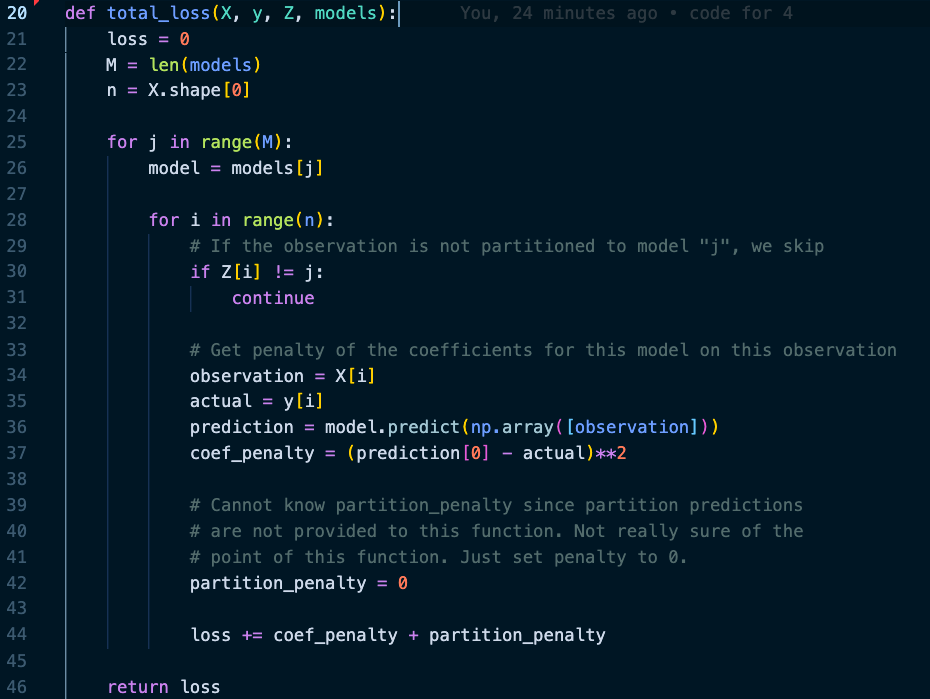
\includegraphics[scale=0.4]{q4c_code1.png}

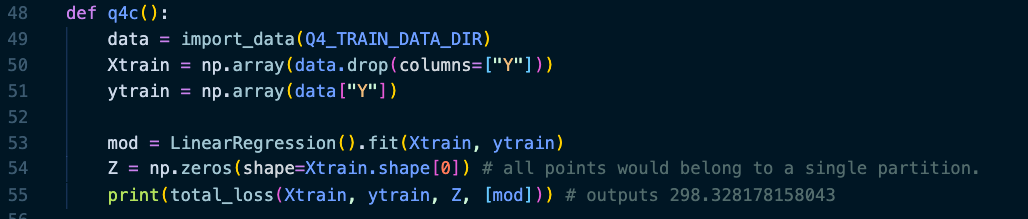
\includegraphics[scale=0.4]{q4c_code2.png}

\subsection*{d}

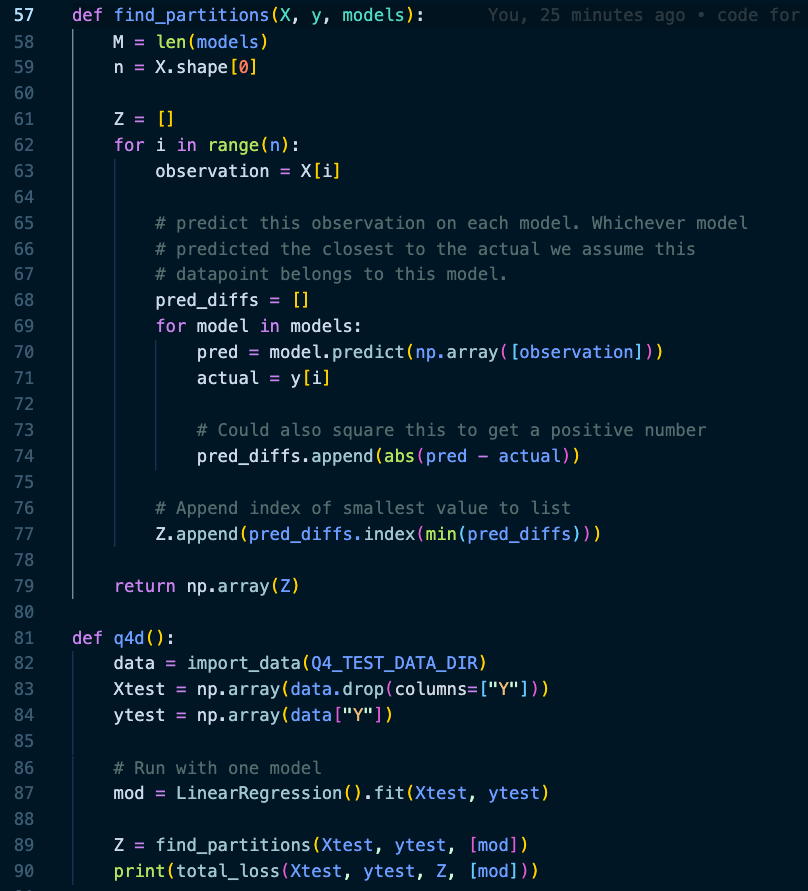
\includegraphics[scale=0.5]{q4d_code1.png}

\newpage
\subsection*{e}

See code for this question here \ref{code:q4e}

\begin{verbatim}
    M  |        train        |        test          |
    5  |  773.2139301322158  |  116.60294714118255  |
    10 |  1226.975556530428  |  190.77503856677967  |
    15 |  1854.7758161852978 |  374.3318184723467   |
    20 |  5245.153194657786  |  924.8003322754047   |
    25 |  3687.1371589765313 |  572.1619888958278   |
    30 |  4150.443300036157  |  703.5325244593158   |
\end{verbatim}

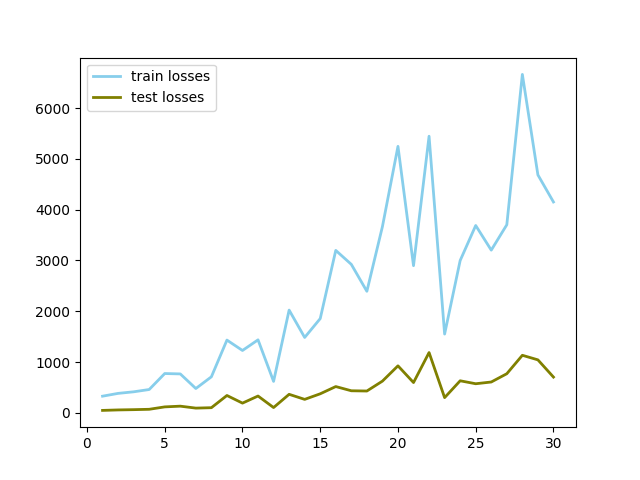
\includegraphics[scale=0.8]{q4e.png}

Based on the results, I would guess that the most reasonable 
value for M is around 6 or 8. Even though the train losses 
were lower when M < 5, the test losses were approximately 
the same for M from 0 to 8 and a lower value for M would be favoured
since each of the models gets trained on more data.

\newpage
\section*{Appendix}

\subsection{q4e}
\label{code:q4e}

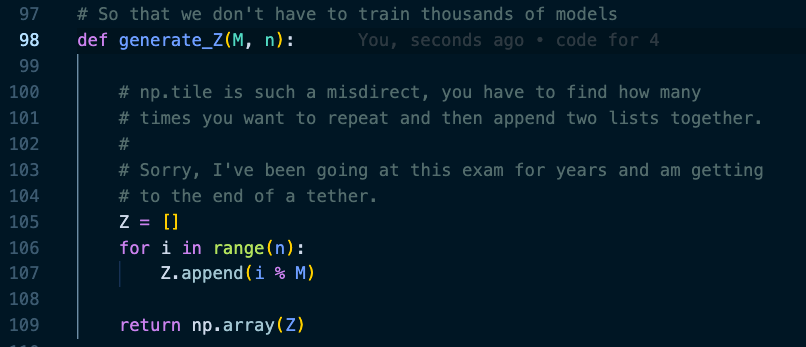
\includegraphics[scale=0.4]{q4e_code1.png}

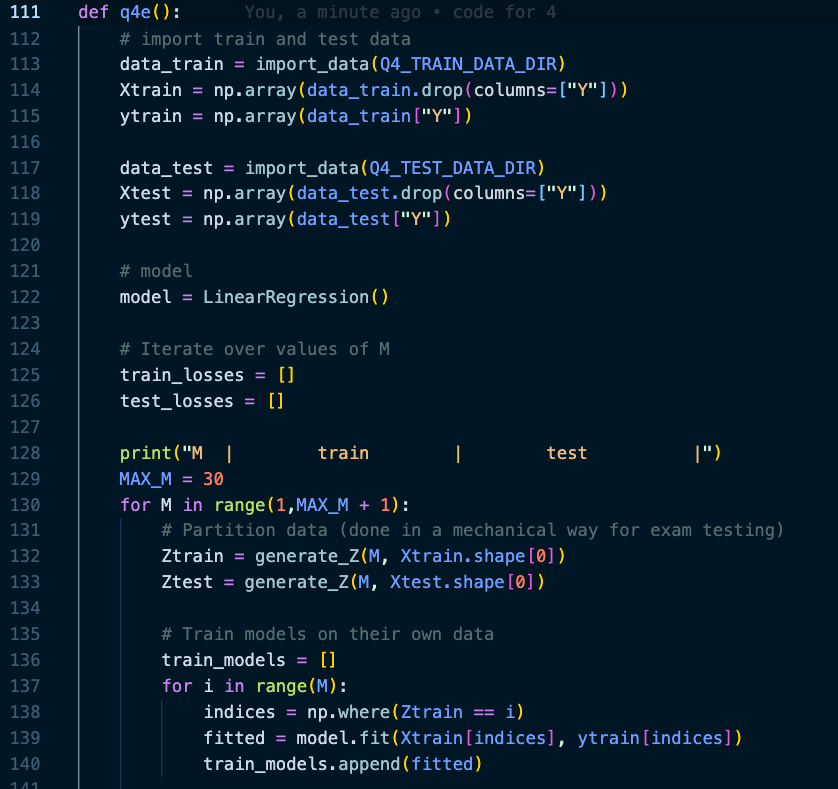
\includegraphics[scale=0.4]{q4e_code2.png}

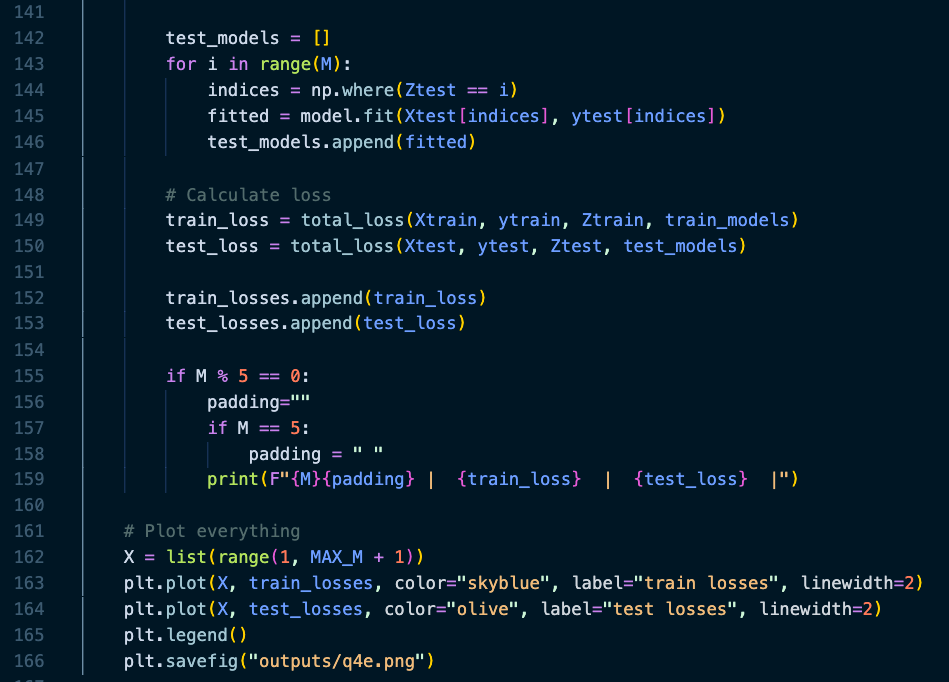
\includegraphics[scale=0.4]{q4e_code3.png}

\end{document}
